\section{Faster and Faster Approximations}
\label{sec:inductive-smoothening}
In this section we would like to improve on the rate of convergence of Theorem~\ref{thm:phase-extraction-jackson-rate}, which we can plug into Algorithm~\ref{alg:prop-sampling-qsp} to achieve further speed-up. We restate an important result about Fourier series here, which we also used in the proof of Theorem~\ref{thm:phase-extraction-jackson-rate}:
\begin{theorem}[Jackson~\cite{jacksonTheoryApproximation1930a}, Corollary 3, p.\ 22]
    \label{thm:jackson-rate}
    If $f : \R \rightarrow \R$ is a $2\pi$-periodic function such that its $p$-th derivative is $K$-Lipschitz continuous, then its Fourier sum $S_d(x)$ of $d$-th degree satisfies
    \begin{align*}
        ||S_d - f||_\R \le K \frac{A_p \log d}{d^{p+1}}
    \end{align*}
    where $A_p$ is a constant depending only on $p$.
\end{theorem}
In our example we took $p = 1$, we smoothed out $\phi_\delta$ so that its first derivative is continuous and we noticed that it is $\frac{2}{\delta^2}$-Lipschitz. This led to $d = \Tilde\bigO\left(\frac{1}{\delta} \sqrt{\frac{1}{\epsilon}}\right)$ to bound the approximation error by $\epsilon$ on the unit circle. However in the application for proportional sampling we could do more: we could smooth out all the derivatives up to some constant $p$, taking advantage of the fact that $\delta = \pi/2$.

\begin{figure*}
    \centering
    \def\dlt{0.4}
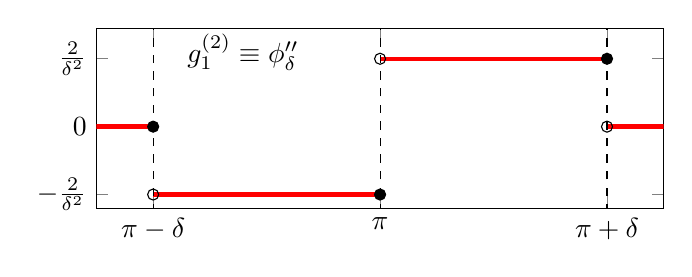
\begin{tikzpicture}
\begin{axis}[
    width=250pt,height=110pt,
    xmin=pi-0.5,xmax=pi+0.5,
    ymin=-1.2,ymax=1.45,
    samples=50,
    xtick={pi-\dlt, pi, pi+\dlt},
    xticklabels={$\pi - \delta$, $\pi$, $\pi + \delta$},
    ytick={-1, 0, 1},
    yticklabels={$-\frac{2}{\delta^2}$, $0$, $\frac{2}{\delta^2}$},
    grid style={line width=.1pt, draw=gray!10}]

    \addplot[red, ultra thick, domain=0:pi-\dlt] (x, 0);
    \addplot[red, ultra thick, domain=pi+\dlt:4] (x, 0);
    \addplot[red, ultra thick, domain=pi-\dlt:pi] (x, -1);
    \addplot[red, ultra thick, domain=pi:pi+\dlt] (x, 1);

    \draw [dashed] (axis cs:{pi-\dlt},-2) -- (axis cs:{pi-\dlt},2);
    \draw [dashed] (axis cs:{pi},-2) -- (axis cs:{pi},2);
    \draw [dashed] (axis cs:{pi+\dlt},-2) -- (axis cs:{pi+\dlt},2);
    
    \node at (axis cs:2.9,1.1) {$g^{(2)}_1 \equiv \phi''_\delta$};

    \addplot[mark=*] coordinates {(pi-\dlt,0)};
    \addplot[mark=o] coordinates {(pi-\dlt,-1)};
    \addplot[mark=*] coordinates {(pi,-1)};
    \addplot[mark=o] coordinates {(pi,1)};
    \addplot[mark=*] coordinates {(pi+\dlt,1)};
    \addplot[mark=o] coordinates {(pi+\dlt,0)};
\end{axis}
\end{tikzpicture}
\undef\dlt
    \def\dlt{0.4}
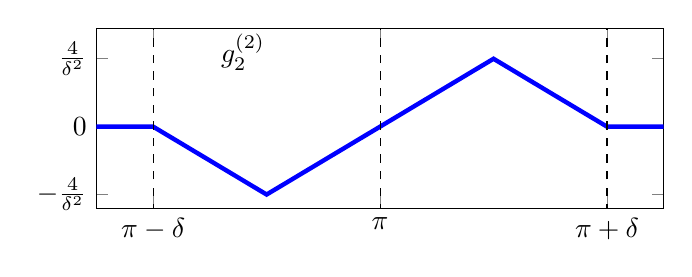
\begin{tikzpicture}
\begin{axis}[
    width=250pt,height=110pt,
    xmin=pi-0.5,xmax=pi+0.5,
    ymin=-1.2,ymax=1.45,
    samples=50,
    xtick={pi-\dlt, pi, pi+\dlt},
    xticklabels={$\pi - \delta$, $\pi$, $\pi + \delta$},
    ytick={-1, 0, 1},
    yticklabels={$-\frac{4}{\delta^2}$, $0$, $\frac{4}{\delta^2}$},
    grid style={line width=.1pt, draw=gray!10}]

    \addplot[blue, ultra thick] coordinates {
        (0, 0) (pi-\dlt, 0) (pi-\dlt/2, -1) (pi+\dlt/2, 1) (pi+\dlt, 0) (4,0)
    };

    \draw [dashed] (axis cs:{pi-\dlt},-2) -- (axis cs:{pi-\dlt},2);
    \draw [dashed] (axis cs:{pi},-2) -- (axis cs:{pi},2);
    \draw [dashed] (axis cs:{pi+\dlt},-2) -- (axis cs:{pi+\dlt},2);
    
    \node at (axis cs:2.9,1.1) {$g^{(2)}_2$};
\end{axis}
\end{tikzpicture}
\undef\dlt
    \def\dlt{0.4}
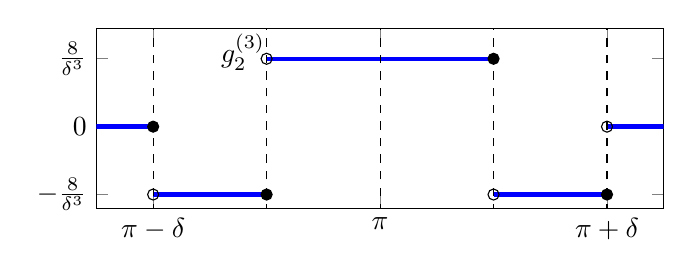
\begin{tikzpicture}
\begin{axis}[
    width=250pt,height=110pt,
    xmin=pi-0.5,xmax=pi+0.5,
    ymin=-1.2,ymax=1.45,
    samples=50,
    xtick={pi-\dlt, pi, pi+\dlt},
    xticklabels={$\pi - \delta$, $\pi$, $\pi + \delta$},
    ytick={-1, 0, 1},
    yticklabels={$-\frac{8}{\delta^3}$, $0$, $\frac{8}{\delta^3}$},
    grid style={line width=.1pt, draw=gray!10}]

    \addplot[blue, ultra thick, domain=0:pi-\dlt] (x, 0);
    \addplot[blue, ultra thick, domain=pi-\dlt:pi-\dlt/2] (x, -1);
    \addplot[blue, ultra thick, domain=pi-\dlt/2:pi+\dlt/2] (x, 1);
    \addplot[blue, ultra thick, domain=pi+\dlt/2:pi+\dlt] (x, -1);
    \addplot[blue, ultra thick, domain=pi+\dlt:4] (x, 0);

    \draw [dashed] (axis cs:{pi-\dlt},-2) -- (axis cs:{pi-\dlt},2);
    \draw [dashed] (axis cs:{pi-\dlt/2},-2) -- (axis cs:{pi-\dlt/2},2);
    \draw [dashed] (axis cs:{pi},-2) -- (axis cs:{pi},2);
    \draw [dashed] (axis cs:{pi+\dlt/2},-2) -- (axis cs:{pi+\dlt/2},2);
    \draw [dashed] (axis cs:{pi+\dlt},-2) -- (axis cs:{pi+\dlt},2);
    
    \node at (axis cs:2.9,1.1) {$g^{(3)}_2$};

    \addplot[mark=*] coordinates {(pi-\dlt,0)};
    \addplot[mark=o] coordinates {(pi-\dlt,-1)};
    \addplot[mark=*] coordinates {(pi-\dlt/2,-1)};
    \addplot[mark=o] coordinates {(pi-\dlt/2,1)};
    \addplot[mark=*] coordinates {(pi+\dlt/2,1)};
    \addplot[mark=o] coordinates {(pi+\dlt/2,-1)};
    \addplot[mark=*] coordinates {(pi+\dlt,-1)};
    \addplot[mark=o] coordinates {(pi+\dlt,0)};
\end{axis}
\end{tikzpicture}
\undef\dlt
    \def\dlt{0.4}
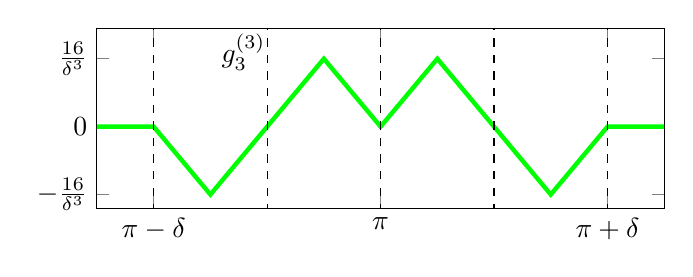
\begin{tikzpicture}
\begin{axis}[
    width=250pt,height=110pt,
    xmin=pi-0.5,xmax=pi+0.5,
    ymin=-1.2,ymax=1.45,
    samples=50,
    xtick={pi-\dlt, pi, pi+\dlt},
    xticklabels={$\pi - \delta$, $\pi$, $\pi + \delta$},
    ytick={-1, 0, 1},
    yticklabels={$-\frac{16}{\delta^3}$, $0$, $\frac{16}{\delta^3}$},
    grid style={line width=.1pt, draw=gray!10}]

    \addplot[green, ultra thick] coordinates {
        (0, 0) (pi-\dlt, 0) (pi-3*\dlt/4, -1) (pi-\dlt/4, 1) (pi, 0) (pi+\dlt/4, 1) (pi+3*\dlt/4, -1) (pi+\dlt, 0) (4,0)
    };

    \draw [dashed] (axis cs:{pi-\dlt},-2) -- (axis cs:{pi-\dlt},2);
    \draw [dashed] (axis cs:{pi-\dlt/2},-2) -- (axis cs:{pi-\dlt/2},2);
    \draw [dashed] (axis cs:{pi},-2) -- (axis cs:{pi},2);
    \draw [dashed] (axis cs:{pi+\dlt/2},-2) -- (axis cs:{pi+\dlt/2},2);
    \draw [dashed] (axis cs:{pi+\dlt},-2) -- (axis cs:{pi+\dlt},2);
    
    \node at (axis cs:2.9,1.1) {$g^{(3)}_3$};
\end{axis}
\end{tikzpicture}
\undef\dlt
    \def\dlt{0.4}
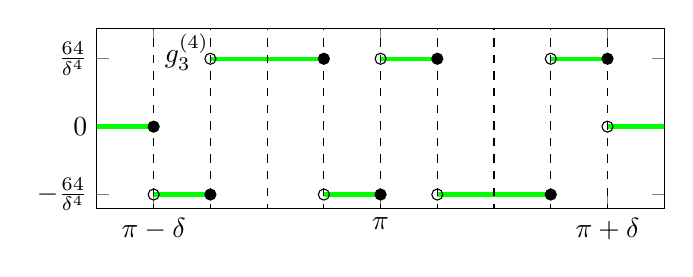
\begin{tikzpicture}
\begin{axis}[
    width=250pt,height=110pt,
    xmin=pi-0.5,xmax=pi+0.5,
    ymin=-1.2,ymax=1.45,
    samples=50,
    xtick={pi-\dlt, pi, pi+\dlt},
    xticklabels={$\pi - \delta$, $\pi$, $\pi + \delta$},
    ytick={-1, 0, 1},
    yticklabels={$-\frac{64}{\delta^4}$, $0$, $\frac{64}{\delta^4}$},
    grid style={line width=.1pt, draw=gray!10}]

    \addplot[green, ultra thick, domain=0:pi-\dlt] (x, 0);
    \addplot[green, ultra thick, domain=pi-\dlt:pi-3*\dlt/4] (x, -1);
    \addplot[green, ultra thick, domain=pi-3*\dlt/4:pi-\dlt/2] (x, 1);
    \addplot[green, ultra thick, domain=pi-\dlt/2:pi-\dlt/4] (x, 1);
    \addplot[green, ultra thick, domain=pi-\dlt/4:pi] (x, -1);
    \addplot[green, ultra thick, domain=pi:pi+\dlt/4] (x, 1);
    \addplot[green, ultra thick, domain=pi+\dlt/4:pi+\dlt/2] (x, -1);
    \addplot[green, ultra thick, domain=pi+\dlt/2:pi+3*\dlt/4] (x, -1);
    \addplot[green, ultra thick, domain=pi+3*\dlt/4:pi+\dlt] (x, 1);
    \addplot[green, ultra thick, domain=pi+\dlt:4] (x, 0);

    \draw [dashed] (axis cs:{pi-\dlt},-2) -- (axis cs:{pi-\dlt},2);
    \draw [dashed] (axis cs:{pi-3*\dlt/4},-2) -- (axis cs:{pi-3*\dlt/4},2);
    \draw [dashed] (axis cs:{pi-\dlt/2},-2) -- (axis cs:{pi-\dlt/2},2);
    \draw [dashed] (axis cs:{pi-\dlt/4},-2) -- (axis cs:{pi-\dlt/4},2);
    \draw [dashed] (axis cs:{pi},-2) -- (axis cs:{pi},2);
    \draw [dashed] (axis cs:{pi+\dlt/4},-2) -- (axis cs:{pi+\dlt/4},2);
    \draw [dashed] (axis cs:{pi+\dlt/2},-2) -- (axis cs:{pi+\dlt/2},2);
    \draw [dashed] (axis cs:{pi+3*\dlt/4},-2) -- (axis cs:{pi+3*\dlt/4},2);
    \draw [dashed] (axis cs:{pi+\dlt},-2) -- (axis cs:{pi+\dlt},2);
    
    \node at (axis cs:2.8,1.1) {$g^{(4)}_3$};

    \addplot[mark=*] coordinates {(pi-\dlt,0)};
    \addplot[mark=o] coordinates {(pi-\dlt,-1)};
    \addplot[mark=*] coordinates {(pi-3*\dlt/4,-1)};
    \addplot[mark=o] coordinates {(pi-3*\dlt/4,1)};
    \addplot[mark=*] coordinates {(pi-\dlt/4,1)};
    \addplot[mark=o] coordinates {(pi-\dlt/4,-1)};
    \addplot[mark=*] coordinates {(pi,-1)};
    \addplot[mark=o] coordinates {(pi,1)};
    \addplot[mark=*] coordinates {(pi+\dlt/4,1)};
    \addplot[mark=o] coordinates {(pi+\dlt/4,-1)};
    \addplot[mark=*] coordinates {(pi+3*\dlt/4,-1)};
    \addplot[mark=o] coordinates {(pi+3*\dlt/4,1)};
    \addplot[mark=*] coordinates {(pi+\dlt,1)};
    \addplot[mark=o] coordinates {(pi+\dlt,0)};
\end{axis}
\end{tikzpicture}
\undef\dlt
    \def\dlt{0.4}
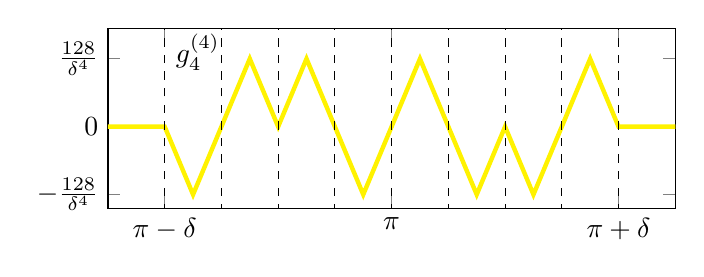
\begin{tikzpicture}
\begin{axis}[
    width=250pt,height=110pt,
    xmin=pi-0.5,xmax=pi+0.5,
    ymin=-1.2,ymax=1.45,
    samples=50,
    xtick={pi-\dlt, pi, pi+\dlt},
    xticklabels={$\pi - \delta$, $\pi$, $\pi + \delta$},
    ytick={-1, 0, 1},
    yticklabels={$-\frac{128}{\delta^4}$, $0$, $\frac{128}{\delta^4}$},
    grid style={line width=.1pt, draw=gray!10}]

    \addplot[yellow, ultra thick] coordinates {
        (0, 0) (pi-\dlt, 0) (pi-7*\dlt/8, -1) (pi-5*\dlt/8, 1) (pi-\dlt/2, 0) (pi-3*\dlt/8, 1) (pi-\dlt/8, -1) (pi+\dlt/8, 1) (pi+3*\dlt/8, -1) (pi+\dlt/2, 0) (pi+5*\dlt/8, -1) (pi+7*\dlt/8, 1) (pi+\dlt, 0) (4,0)
    };

    \draw [dashed] (axis cs:{pi-\dlt},-2) -- (axis cs:{pi-\dlt},2);
    \draw [dashed] (axis cs:{pi-3*\dlt/4},-2) -- (axis cs:{pi-3*\dlt/4},2);
    \draw [dashed] (axis cs:{pi-\dlt/2},-2) -- (axis cs:{pi-\dlt/2},2);
    \draw [dashed] (axis cs:{pi-\dlt/4},-2) -- (axis cs:{pi-\dlt/4},2);
    \draw [dashed] (axis cs:{pi},-2) -- (axis cs:{pi},2);
    \draw [dashed] (axis cs:{pi+\dlt/4},-2) -- (axis cs:{pi+\dlt/4},2);
    \draw [dashed] (axis cs:{pi+\dlt/2},-2) -- (axis cs:{pi+\dlt/2},2);
    \draw [dashed] (axis cs:{pi+3*\dlt/4},-2) -- (axis cs:{pi+3*\dlt/4},2);
    \draw [dashed] (axis cs:{pi+\dlt},-2) -- (axis cs:{pi+\dlt},2);
    
    \node at (axis cs:2.8,1.1) {$g^{(4)}_4$};
\end{axis}
\end{tikzpicture}
\undef\dlt
    \caption{Construction of the fourth derivative of $g_4 \in C^4$. To construct the derivative of the next function, we linearize the `last' derivative in order to make it continuous, and we do so by replacing the rectangles with triangles of the same area, so that the integral over $I = (\pi - \delta, \pi + \delta)$ is preserved. In order to obtain $g_4$, we will integrate four times, keeping in mind that every derivative has value $0$ at the origin, except for the first one, which has value $1/\pi$.}
    \label{fig:function-smoothening-1}
\end{figure*}

\begin{figure}
    \centering
    \def\dlt{0.4}
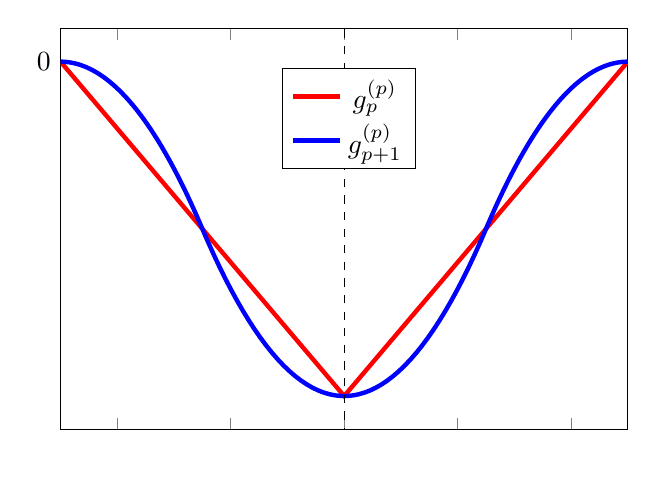
\begin{tikzpicture}
\begin{axis}[
    width=250pt,height=190pt,
    xmin=-0.5,xmax=+0.5,
    ymin=-0.55,ymax=0.05,
    samples=50,
    xtick={},
    xticklabels={},
    ytick={0},
    yticklabels={$0$},
    grid style={line width=.1pt, draw=gray!10},
    legend style={at={(0.39,0.9)}, anchor=north west}]

    \addplot[red, ultra thick] coordinates {
        (-0.5, 0) (0, -0.5) (0.5,0)
    };

    \addplot[blue, ultra thick, domain=-0.5:-0.25] (x, {-4*x*x-4*x-1});
    \legend{$g^{(p)}_p$, $g^{(p)}_{p+1}$}
    \addplot[blue, ultra thick, domain=-0.25:0.25] (x, {4*x*x-0.5});
    \addplot[blue, ultra thick, domain=0.25:0.5] (x, {-4*x*x+4*x-1});
    

    \draw [dashed] (axis cs:{0},-2) -- (axis cs:{0},2);
    
    \node at (axis cs:2.9,1.1) {$g^{(3)}_3$};
\end{axis}
\end{tikzpicture}
\undef\dlt
    \caption{Comparison between a triangle and its first-order smoothing. If this is the $j$-th triangle of $g^{(p)}_{p+1}$, then the interval of the plot is $I^{p-1}_j$, which is split into the two intervals $I^p_{2j}, I^p_{2j+1}$. One can see that the difference of the two functions is odd in each of the two sub-intervals, and even in $I^{p-1}_j$.}
    \label{fig:function-smoothening-parabola}
\end{figure}

We generalize the smoothing procedure shown in Section~\ref{sec:phase-extraction-problem}: one can see that $\phi'_\delta$ is a piecewise linear function.
\begin{claim}
    For $p \ge 1$, we can construct $g_p \in C^p$ that is $2\pi$-periodic, and
    \begin{align}
        \label{eq:general-construction-identity-condition}
        g_p(x) = \frac{x}{\pi}
    \end{align}
    for every $x \in (-\pi + \delta, \pi - \delta)$.
\end{claim}

\begin{proof}
    Note that $g_1 \equiv \phi_\delta$ gives a base for our inductive construction. First of all, Eq.~(\ref{eq:general-construction-identity-condition}) holds iff the derivatives of $g_p$ satisfy:
    \begin{align}
        \label{eq:smoothening-derivative-values}
        g^{(k)}_p(x) & = 
        \begin{cases}
            \frac{1}{\pi} & k = 1 \\
            0 & k \neq 1
        \end{cases}
    \end{align}
    for $x \in (-\pi + \delta, \pi - \delta)$ and every $k \ge 0$. By this condition, we are only allowed to change the behaviour of the function outside of this domain, thus from now on we will only consider the interval $I = (\pi-\delta, \pi+\delta)$.
    
    Starting from $g^{(1)}_1$, which is continuous and piecewise linear, its derivative, $g^{(2)}_1$ will be piecewise constant, i.e., its integral will be given by a sequence of rectangles (Figure~\ref{fig:function-smoothening-1}, top left). We construct the second derivative of the next function $g^{(2)}_2$ by replacing the rectangles of $g^{(1)}_2$ by triangles of the same area (Figure~\ref{fig:function-smoothening-1}, top right). Then $g^{(3)}_2$ will be again piecewise constant, where the number of intervals in which this function is subdivided is twice the intervals of our starting function $g^{(2)}_1$. In general, $g^{(p)}_{p+1}$ will be piecewise constant, $g^{(p+1)}_{p+1}$ is obtained with the above procedure, and its pieces divide $I$ into $2^p$ equal segments. At this point, $g_p$ is easily defined by integrating the constructed derivatives $p+1$ times, with boundary conditions given by Eq.~(\ref{eq:smoothening-derivative-values}):
    \begin{align*}
        g_{p+1}(x) = \int_0^x \left( \frac{1}{\pi} + \underbrace{\int_0^x \cdots \int_0^x}_{p} g^{(p+1)}_{p+1}(x) \ dx^p \right) dx\ .
    \end{align*}
    Figure~\ref{fig:function-smoothening-1} shows the construction of the fourth derivative of $g_4$. We now prove all the claimed properties: $g_p \in C^p$ by construction, and we never changed the derivatives within $\pm (\pi - \delta)$, thus Eq.~(\ref{eq:smoothening-derivative-values}) is preserved (and so is also (\ref{eq:general-construction-identity-condition})).
    We only need to prove periodicity: the key here is to notice that $g^{(2)}_p$ satisfies
    \begin{align*}
        \int_I g^{(2)}_p(t) \ dt = 0 \ ,
    \end{align*}
    implying that $g^{(1)}_p$ is $\frac{1}{\pi}$ at the boundaries of $I$. This because $g^{(2)}_p$ has the same form as $g^{(2)}_1$ in Figure~\ref{fig:function-smoothening-1}, except for the fact that, instead of having two opposite rectangles, we have two opposite (smoother) shapes which will cancel out with one another in the integral (in the case of $p = 2$, these shapes are the triangles as in Figure~\ref{fig:function-smoothening-1}, top right). This shows that $g^{(1)}_p$ is $2\pi$-periodic. It is now sufficient to prove
    \begin{align}
        \label{eq:smoothening-ultimate-integral-condition}
        g_p(2\pi) - g_p(0) = \int_0^{2\pi} g^{(1)}_p(t) \ dt = 0
    \end{align}
    in order to prove periodicity of $g_p$.
    This is already true for $p = 1$, by design: in this case the shape of $g^{(1)}_1$ in $I$ is one big triangle pointing downwards, whose area was chosen in order to satisfy (\ref{eq:smoothening-ultimate-integral-condition}).

    For $p > 1$, this triangle is replaced by a smoother shape, and it is sufficient to prove that such shape has the same area as the original triangle in order to preserve the above integral. Thus we prove the following by induction:
    \begin{align*}
        \int_I g^{(1)}_{p+1}(t) - g^{(1)}_p(t) \ dt = 0
    \end{align*}
    so that by telescoping and linearity of integral the claim will follow. We introduce some notation: for $0 \le j < 2^k$, $I^k_j$ is the $j$-th slice of $I$ (starting from its left endpoint $\pi - \delta$) after dividing it into $2^k$ sub-intervals. Notice that it holds that $I^{k-1}_j = I^k_{2j} \cup I^k_{2j+1}$, for $0 \le j < 2^{k-1}$. When we say that a function is even (odd) in some interval, we mean that the function restricted to that interval is symmetric (anti-symmetric) with respect to the middle point.
    
    As a base for an inductive argument, one can see that the function $g^{(p)}_{p+1} - g^{(p)}_p$ is odd in $I^p_j$, for every $j$: this because $g^{(p)}_p$ is the side of a triangle in $I^p_{j}$, $g^{(p)}_{p+1}$ is the side of a parabolic bell and we can directly check that the difference is odd in $I^p_{j}$ (see Figure~\ref{fig:function-smoothening-parabola}).
    
    Assuming that $g^{(k)}_{p+1} - g^{(k)}_p$ is odd in $I^k_j$ for every $j$ and some $1 < k \le p$, we have that
    \begin{align*}
        \int_{L(I^k_j)}^{R(I^k_j)} g^{(k)}_{p+1}(t) - g^{(k)}_p(t) \ dt = 0 \ ,
    \end{align*}
    where $L(J), R(J)$ are, respectively, the left and right endpoints of an interval $J$. The function $g^{(k)}_p$ is a sequence of (smoothed) triangles in $I$, but this shape must be equal to $0$ at the endpoints: this because these shapes are symmetric and all equal up to sign by construction and the left endpoint of the leftmost shape must preserve continuity with the constant function outside of $I$, in both $g^{(k)}_p$ and its smoothed version $g^{(k)}_{p+1}$. Hence, at the base of the shapes the difference is $0$.
    One of $L(I^k_j), R(I^k_j)$, corresponds to one of the base points of the shape, while the other is the peak (which one depends on whether $I^k_j$ contains the first or second half of the shape, i.e., the parity of $j$). By oddness in this interval, also at the peak the difference is $0$. Considering the leftmost shape, the function $g^{(k)}_{p+1} - g^{(k)}_p$ is even in $I^{k-1}_0 = I^k_0 \cup I^k_1$. Therefore,
    \begin{align*}
        g^{(k-1)}_{p+1} - g^{(k-1)}_p & = \int_{0}^x g^{(k)}_{p+1}(t) - g^{(k)}_p(t) \ dt \\
        & = \int_{L(I^k_0)}^x g^{(k)}_{p+1}(t) - g^{(k)}_p(t) \ dt \\
        & = \int_{R(I^k_0)}^x g^{(k)}_{p+1}(t) - g^{(k)}_p(t) \ dt \ ,
    \end{align*}
    and the last expression is clearly odd in $I^{k-1}_0$, since $R(I^k_0)$ is the middle point.
    
    By a simple induction on $j$ the result can be extended to every shape, implying that $g^{(k-1)}_{p+1} - g^{(k-1)}_p$ is odd in $I^{k-1}_j$ for every $j$, and in particular, $g^{(1)}_{p+1} - g^{(1)}_p$ is odd in $I^1_0, I^1_1$, and both integrals cancel out, giving zero also on their union, which is the whole interval $I$.
\end{proof}
All we need now is to bound the Lipschitz constant for $g^{(p)}_p$: we already know that $g^{(1)}_1$ is $K_1$-Lipschitz with
\begin{align*}
    K_1 = \frac{2}{\delta^2}
\end{align*}
since its derivative $g^{(2)}_1$ is bounded by this number in absolute value. If $K_p$ is the Lipschitz constant of $g^{(p)}_p$, then
$$K_p = \sup |g^{(p+1)}_p| \ .$$
In order to obtain the same integral when we transform the rectangles into triangles, we need twice the height, thus the triangles of $g^{(p+1)}_{p+1}$ are as high as $2 K_p$. The slopes of these triangles are then $2 K_p$ over the length of a single segment which is $\frac{2 \delta}{2^{p+1}}$. Therefore, the Lipschitz constant for $g^{(p+1)}_{p+1}$ is
\begin{align*}
    K_{p+1} = \frac{2 K_p 2^{p+1}}{2 \delta} = \frac{K_p 2^{p+1}}{\delta} \ ,
\end{align*}
and this recurrence relation has unique solution
\begin{align}
    \label{eq:lipschitz-constant-recurrence-solution}
    K_p = \frac{\sqrt{2}^{p(p+1)}}{\delta^{p+1}} \ .
\end{align}
In conclusion, we can now use Theorem~\ref{thm:jackson-rate} to extend Theorem~\ref{thm:phase-extraction-jackson-rate} with a similar argument.
\begin{theorem}
    \label{thm:phase-extraction-jackson-rate-enhanced}
    Let $p > 0$ be a fixed constant. The function $\bar{g}_p : U(1) \rightarrow \R$ defined as
    \begin{align*}
        \bar{g}_p(e^{ix}) = g_p(x)
    \end{align*}
    for every $x \in \R$ can be $\epsilon$-approximated on the unit circle using a polynomial of degree
    \begin{align*}
        d = \Tilde{\bigO}\left(\frac{A_p \sqrt{2}^p}{\delta} \left(\frac{1}{\epsilon}\right)^{\frac{1}{p+1}} \right).
    \end{align*}
\end{theorem}
As a Corollary, for a constant $p$ Algorithm~\ref{alg:prop-sampling-qsp} can be done in only
\begin{align*}
    \Tilde{\bigO}\left( \frac{1}{\bar{c}^{\frac{1}{2} + \frac{1}{p}}} \sqrt[p]{\frac{1}{\epsilon}} \right)
\end{align*}
total oracle queries.